\section{PCB Design}\label{sec:PCB}
\todo[color=c05c,inline]{testing the colors}

To be able to test the proposed topology,
a Printed Circuit Board (PCB) had to be made.
We started out designing a simple two stage layout,
and ended up manufacturing a multi stage version.

\subsection{Two Stage PCB}
To get familiar with designing power electronics PCBs,
we started out designing a two stage version of the proposed topology.
Because we already had some familiarities with EAGLE from previous projects,
we used EAGLE for the first design attempts.
The finished design can be seen in Figure \ref{fig:2nxeagle}.

\begin{figure}[H]
	\begin{center}
	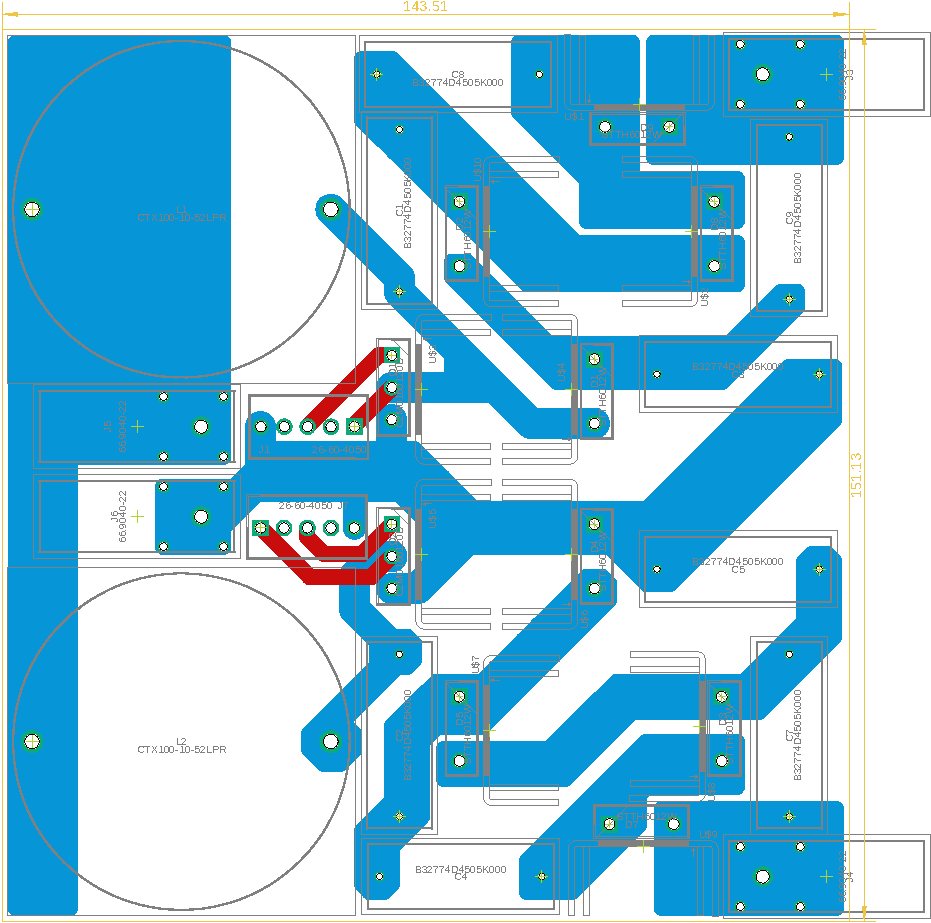
\includegraphics[width=0.6\textwidth]{figures/05cPCBdesign/2NX_interleaved_boost_converter_EAGLE_BY_DANIEL.pdf}
	\end{center}
	\caption{PCB Layout for a two stage 2NX Interleaved Boost Converter}
	\label{fig:2nxeagle}
\end{figure}

The red traces are logical signals,
located on the top layer of the PCB,
blue are power traces located on the bottom layer.
The power traces can be observed to be broader than the logic,
and were drawn as polygons,
to use the biggest available surface area.
The logical signals are designed to be as short as possible
and to be located as far from the power traces as possible,
to minimize interference.

Precautions were made in respect to the method of manufacturing,
because acute angles between two legs of a trace can lead to cracks in the trace when etching.
To prevent this from happening,
more copper was added in the areas in question to create obtuse angles.
A detailed view of this can be seen in Figure \ref{fig:2nxeagledetail}.
\begin{figure}[H]
	\begin{center}
	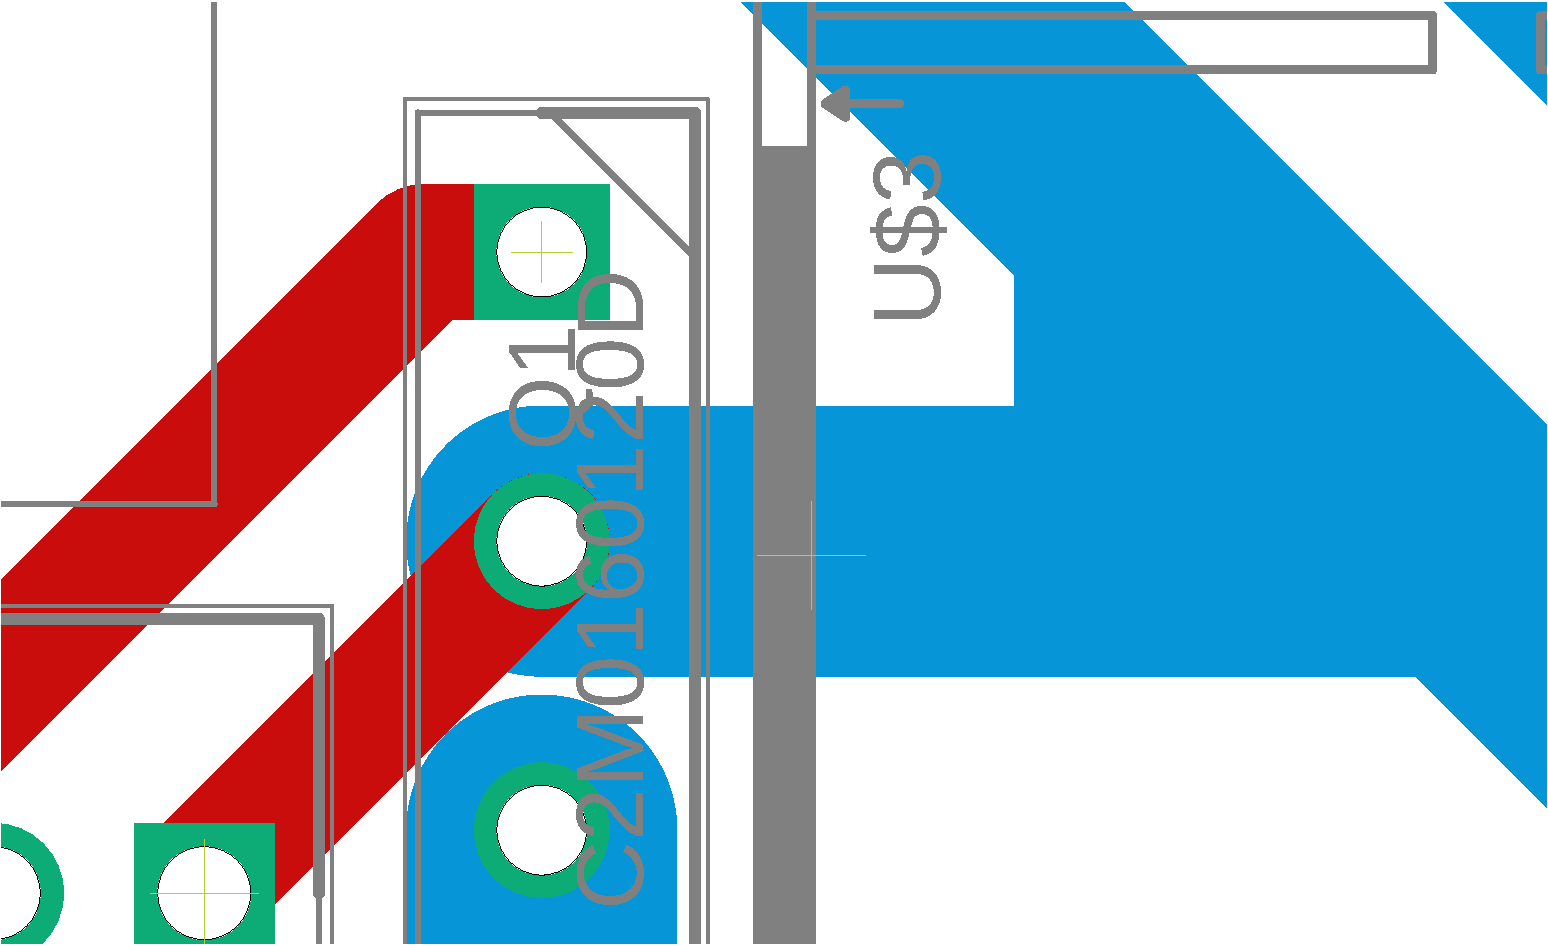
\includegraphics[width=0.6\textwidth]{figures/05cPCBdesign/2NX_interleaved_boost_converter_EAGLE_BY_DANIEL_DETAIL.pdf}
	\end{center}
	\caption{Detailed view of PCB Layout}
	\label{fig:2nxeagledetail}
\end{figure}

\subsection{Multi Stage PCB}\label{sub:3sPCB}
To lessen our workload our supervisor put us into contact with Sagar Mahajan \todo[color=c05c]{cite to his linkedin?},
who already created a layout for the multilevel converter.
We touched up a little bit on the layout to make it producible with the university's equipment,
but the main layouting was not done by us.
The PCB layout can be seen in Figure \ref{fig:2nxDiptrace}.

\begin{figure}[H]
	\begin{center}
	\includegraphics[height=0.6\textwidth,angle=90]{"figures/05cPCBdesign/DipTrace PCB - 2NX_interleaved_DANIEL_EDIT"}
	\end{center}
	\caption{PCB Layout for a multi stage 2NX Interleaved Boost Converter}
	\label{fig:2nxDiptrace}
\end{figure}

As this layout was done in DipTrace,
the colours used differ from the colours used by EAGLE.
Here light red are the copper traces on the bottom layer.
No traces exist on the top layer,
and therefore no layer separation between power and logic is made.

\todo[color=c05c,inline]{something about diptrace, and collaboration with Sagar}